\section{Working Principles}
\label{sec:working_principles}

\acrfull{csacs} can be divided into two main categories based on the atomic element they use and the operating principle they follow.
In this section, we will explore and highlight the key components and contrasting approaches of these two families of \acrshort{csacs}, namely:

\begin{itemize}
  \item \acrfull{modr}, based on \acrfull{rb}
  \item \acrfull{cpt}, based on \acrfull{cs}
\end{itemize}

As we will see, the two technologies have analogous structures, but they differ in the physics package, which is the core of the clock.

\subsection{General overview of a CSAC}
\label{subsec:general_overview}

Before proceeding analyzing in detail the components of a \acrshort{csac}, it's important to understand the general idea that governs its operation.

With respect to traditional quartz oscillators, \acrshort{csacs} exploit the use of a close loop control system to stabilize the frequency of the local oscillator to the atomic transition frequency.
In other words, \acrshort{csacs} leverage the intrinsic stability of atomic transitions to discipline an oscillating circuit based on a vibrating quartz crystal.
Many of the instabilities that affect traditional oscillators, such as temperature sensitivity, aging, and vibration sensitivity (common in classical quartz oscillators), are mitigated by relining on atomic transitions that by their nature are more stable and less sensitive to external factors.

\paragraph{The Building Blocks}

From a functional perspective, a \acrshort{csac} can be broken down into three main blocks, each with a specific role in the system:

\begin{itemize}
    \item \acrfull{pp}: it can be considered the heart of the clock. It contains a vapor cell where the atomic excitation and interrogation take place.
    \item \acrfull{cl}: it can be considered the brain of the clock. It constantly analyzes signals from the physics package and uses this information to fine-tune the frequency of the local oscillator.
    \item \acrfull{lo}: it's the effective source of the clock. Given its intrinsic instabilities, it's constantly disciplined by the control loop to lock its frequency to a known multiple of the atomic transition frequency.
\end{itemize}

Notice that a fourth block is also present in the system, that is the Frequency Synthesizer (FS), which takes the LO's frequency and multiplies it by a known factor to match the range of frequencies needed to interact with the atoms within the physics package.
For the sake of simplicity, we will not delve into the details of the FS in this section, limiting our analysis to the PP, CL, and LO.

The mentioned components are arranged in a closed-loop system, as illustrated in Figure \ref{fig:CSAC-general-overview}.

\begin{figure}[H]
    \centering
    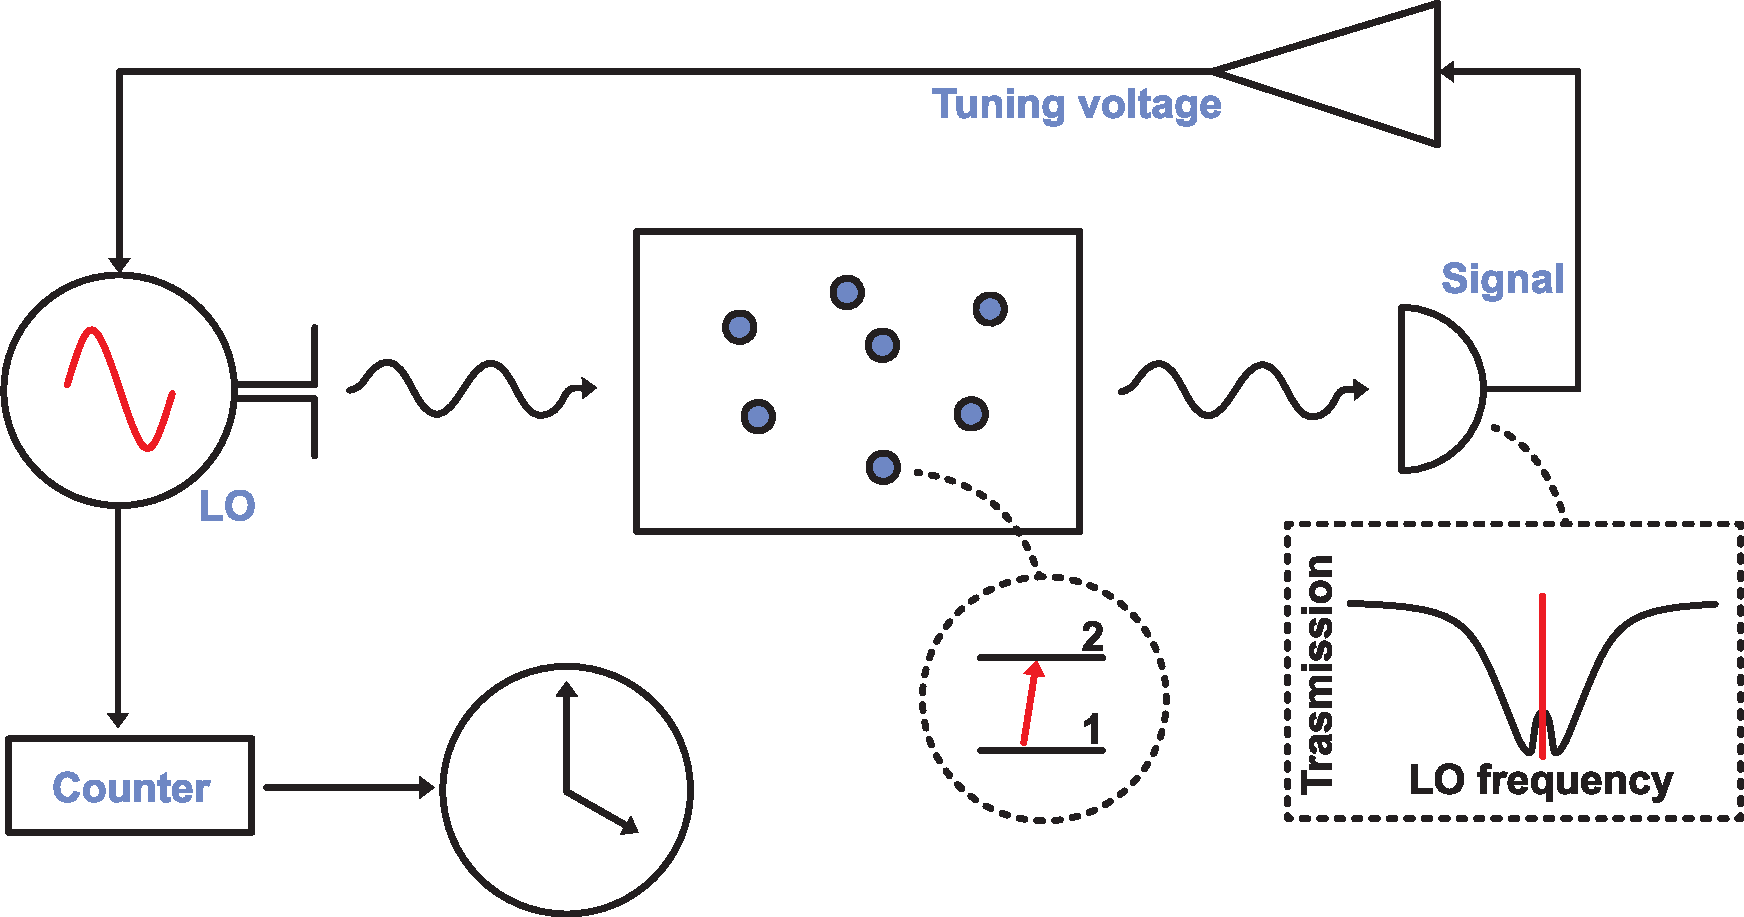
\includegraphics[width=0.7\textwidth, max width=\linewidth]{pdf/CSAC-scheme.pdf}
    \caption{General overview of a \acrshort{csac}}
    \label{fig:CSAC-general-overview}
\end{figure}

In the following sections, we will go through each main block of the \acrshort{csac}, highlighting their fundamental physics and explaining their role in the general framework of the clock.
In Section \ref{sec:performances_and_limitations}, all the limitations and bottleneck associated to each components will be discussed, analyzing their impact on the overall performance of the clock.

\subsection{Physics Package (PP)}
\label{subsec:physics_package}

The \acrfull{pp} is the core component of the \acrshort{csac}, where the atomic excitation and interrogation take place.

Its function is to compare the frequency of the local oscillator with the atomic transition frequency and generate a signal that measures the difference between the two.
From a logical point of view, a generic PP receive as input the local oscillator frequency, and generate as output an electric signal that is sent to the control loop.
Electric power to excite the atoms and thermal power to maintain a steady temperature are also provided to the PP to ensure proper operation.

One of the keys in the stability of a \acrshort{csac}, lies in the capacity of the PP to generate a stable and accurate source of energy required for the excitation of the atoms, which leads to a stable and accurate signal for the control loop.

As we have mentioned at the beginning of this section (Section \ref{sec:working_principles}), \acrshort{csacs} can be divided into two main families based on the atomic element they use and the operating principle they follow.
In the following subsections (Subsections \ref{sssec:MODR} \& \ref{sssec:CPT}), we will delve into the specific architecture for the PP of the two main families of \acrshort{csacs}, namely the one based on \acrfull{modr} and the one based on \acrfull{cpt}.

\subsubsection{Microwave Optical Double-Resonance (MODR)}
\label{sssec:MODR}

In a \acrshort{pp} based on \acrfull{modr}, a vapor gas cell is irradiated simultaneously by a microwave signal (coming from the local oscillator) and a high frequency signal (coming from a laser source).
The combination of the two acting on the \acrfull{rb} atoms inside the cell allows understanding whether the local oscillator is in resonance with the atomic transition frequency or not.

In order to better visualize the operation of a MODR-based \acrshort{csac}, we leave here a schematic representation of its PP (Figure \ref{fig:MODR-physics-package-scheme}).

\begin{figure}[H]
    \centering
    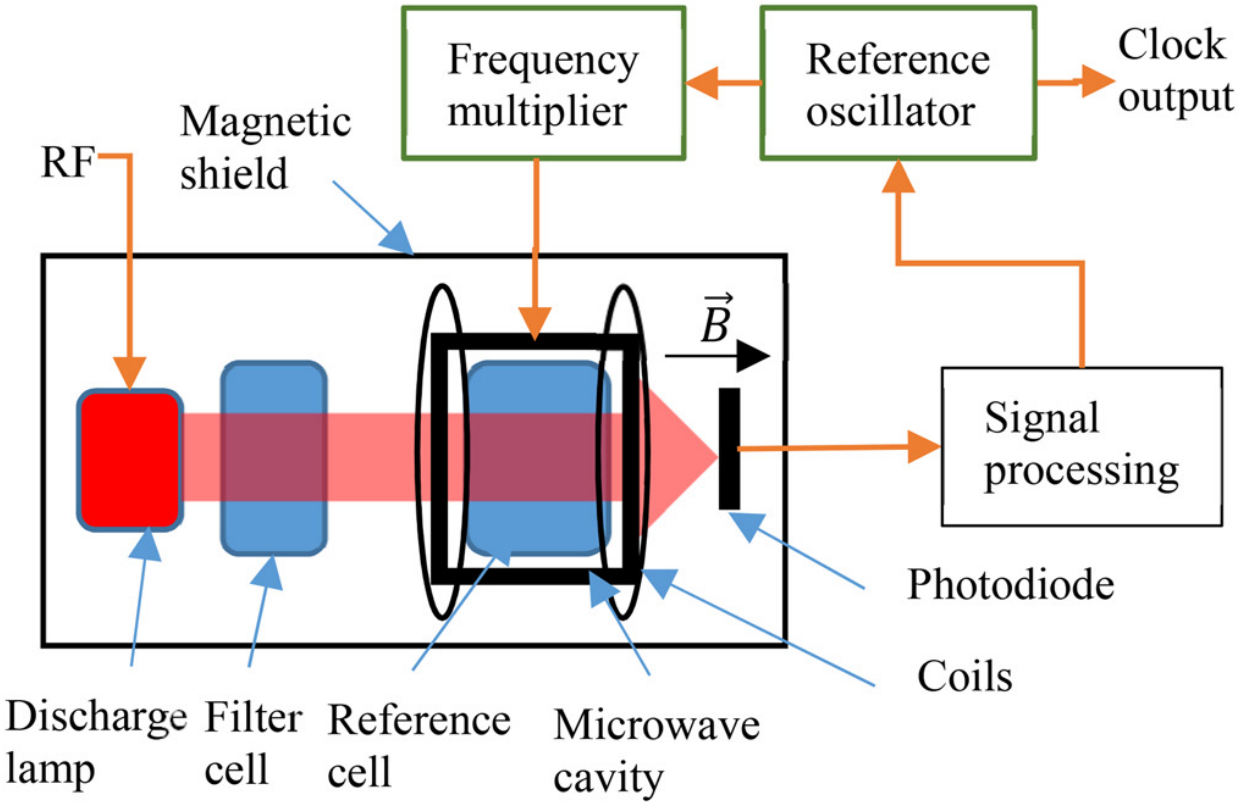
\includegraphics[width=0.6\textwidth, max width=\linewidth]{img/MODR-phisics-package-scheme.png}
    \caption{
        MODR-based \acrshort{csac} scheme.
        Source \cite{Kitching-2018}.
    }
    \label{fig:MODR-physics-package-scheme}
\end{figure}

\paragraph{Target Electron Transitions of Rubidium (Rb)}

In case of PP based on MODR, the vapor gas cell (also called reference cell) is typically filled with \acrfull{rb} ($^{87}Rb$) atoms.
$Rb$ is an alkaline metal with a relatively simple electronic structure, defined as $[Kr]5s^1$.
Its first ionization energy is $4.177 eV$, and the valence electron can be exited using relatively low energy photons.
For these reasons, $Rb$ is widely used in atomic clocks, as it allows for precise manipulation of the valence electron while containing the energy required for the excitation.

In particular, by recalling the quantum energy levels of $^{87}Rb$ (defined by quantum effects and interactions between the electron and the nucleus), we can better define our working frame for the MODR architecture.
Three different transitions are of interest regarding the $^{87}Rb$ atom\footnote{A more comprehensive analysis of the $5S$ \& $5P$ energy levels of $^{87}Rb$ can be found in the Appendix \ref{appendix:Rubidium-energy-levels}.}:

\begin{enumerate}[label = Rb.\Roman*, ref = Rb.\Roman*, leftmargin = *]
    \item \label{itm:Rb-I} $5^2S_{1/2} \quad F=1 \rightarrow 5^2S_{1/2} \quad F=2$: $\approx 6.8GHz$
    \item \label{itm:Rb-II} $5^2S_{1/2} \quad F=1 \rightarrow 5^2P_{1/2}$: $\approx 795^{-}nm$
    \item \label{itm:Rb-III} $5^2S_{1/2} \quad F=2 \rightarrow 5^2P_{1/2}$: $\approx 795^{+}nm$
\end{enumerate}

Notice that the transition $5^2S_{1/2} \rightarrow 5^2P_{1/2}$, of $\approx 795nm$, is usually refereed to as \textit{D1 line}.

As we will see in the following paragraphs, the only transitions that will excite the atoms in the reference cell are \ref{itm:Rb-I} and \ref{itm:Rb-II}.
Transition \ref{itm:Rb-III} is in fact a non-targeted transition that will be filtered out by the system before reaching the reference cell.


\paragraph{Pumping Source}

Having defined our working frame in terms of electron transitions of $^{87}Rb$, we can now step into understanding the mechanism used to excite the atoms in the reference cell.

In a MODR-based \acrshort{csac}, the pumping source is typically a \textit{bulb lamp} (also refereed to as \textit{discharge lamp}, see Figure \ref{fig:MODR-physics-package-scheme}) containing $^{87}Rb$ atoms that after being excited to a higher energy level by an external power source, they decay back to the ground energy level emitting photons.

Since there is no control over the pumping process inside the bulb lamp, more than one transition can be excited.
This means that the lamp will emit photons corresponding to different transitions of the $^{87}Rb$ atoms, including among the others \ref{itm:Rb-II} and \ref{itm:Rb-III} transitions.
However, the photons coming from the \ref{itm:Rb-III} transition are not of interest for the operation of the \acrshort{csac}, and they need to be filtered out.
To do so, a filter cell of $^{85}Rb$ is used since the transition energy of \ref{itm:Rb-III} is almost exactly the same as the transition energy $5^2P_{1/2} \quad F=3 \rightarrow 5^2P$ in $^{85}Rb$.

In the end, from the bulb lamp, the reference cell of the system will receive only photons associated with the \ref{itm:Rb-II} transition.


\paragraph{Electrons Excitation and Interrogation}

Having explained the excitation source, we can now proceed understanding how this energy is used over the atoms present in the \textit{reference cell} (see Figure \ref{fig:MODR-physics-package-scheme}, also refereed to as \textit{vapor gas cell}) and in particular what's the cycle that electrons are forced to.

For the simplicity of explanation, we will consider the different stages of the electrons as if they happen in a temporal sequence.
However, it's important to remind that these stages are not sequential but they happen simultaneously.

We can define three different stages in the cycle of the electrons:

\begin{itemize}
    \item Optical pumping (population inversion and decay): the laser source coming from the bulb lamp excites the atoms to a higher energy level and a population inversion is created between the two hyperfine states $5S_{1/2} F=1$ and $5S_{1/2} F=2$.
    \item Microwave excitation: the microwave signal coming from the local oscillator excites the atoms and, if it's in resonance with the \ref{itm:Rb-I} transition, it force the population accumulated in the $5S_{1/2} F=2$ state to fall back to the $5S_{1/2} F=1$ state.
    \item Optical pumping (interrogation): the same laser used for population inversion is now used to interrogate the atoms and understand if the microwave signal was in resonance with \ref{itm:Rb-I} transition or not.
\end{itemize}

To better understand the cycle of the electrons, we can refer to Figure \ref{fig:MODR-steps}.

\begin{figure}[H]
    \centering

    \begin{minipage}[t]{0.3\linewidth}
        \centering
        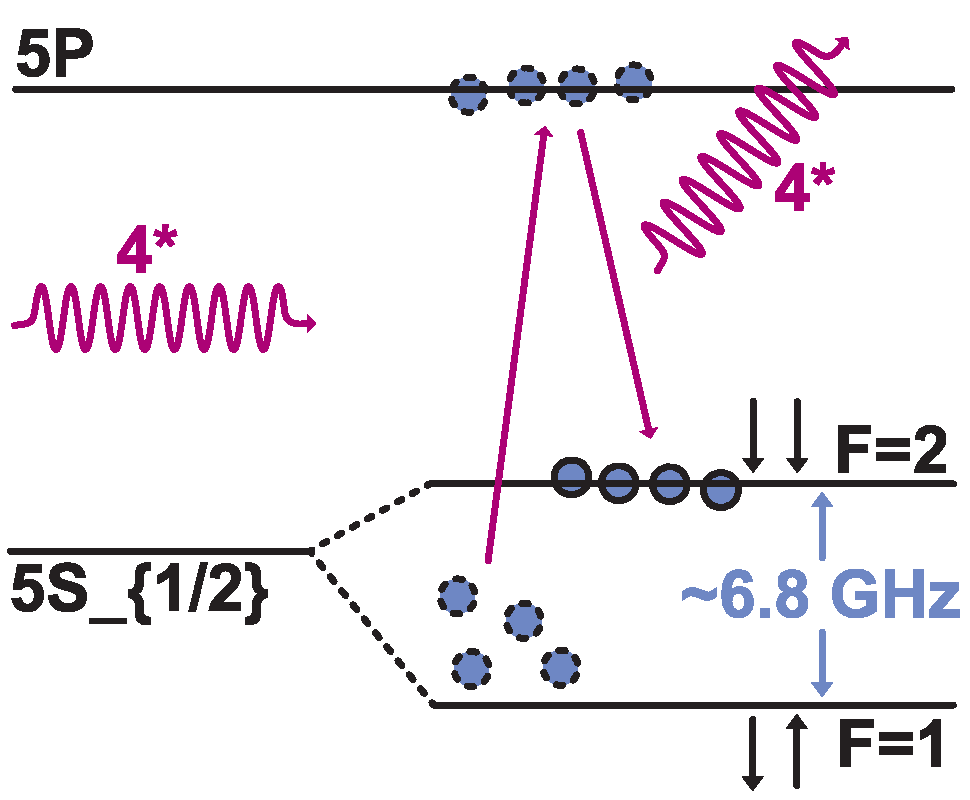
\includegraphics[width=\linewidth]{pdf/MODR/pumping-decay.pdf}
        \caption{Population inversion and decay.}
        \label{fig:MODR-pumping-decay}
    \end{minipage}
    %
    \hfill
    %
    \begin{minipage}[t]{0.3\linewidth}
        \centering
        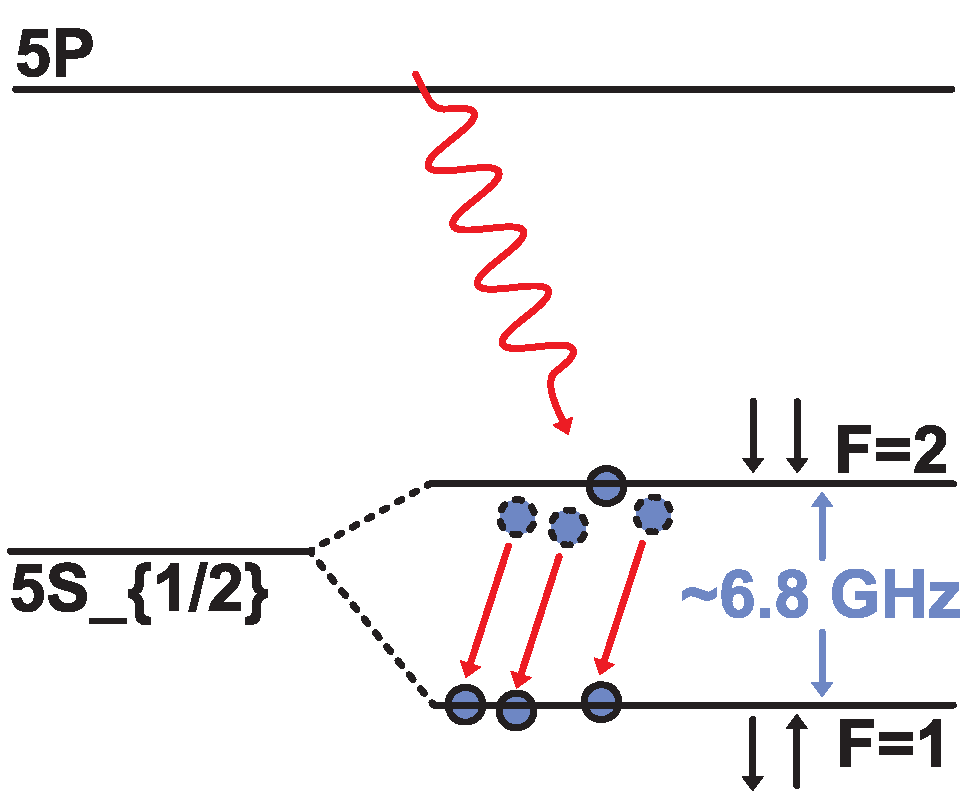
\includegraphics[width=\linewidth]{pdf/MODR/microwave.pdf}
        \caption{Microwave excitation.}
        \label{fig:MODR-microwave}
    \end{minipage}
    %
    \hfill
    %
    \begin{minipage}[t]{0.3\linewidth}
        \centering
        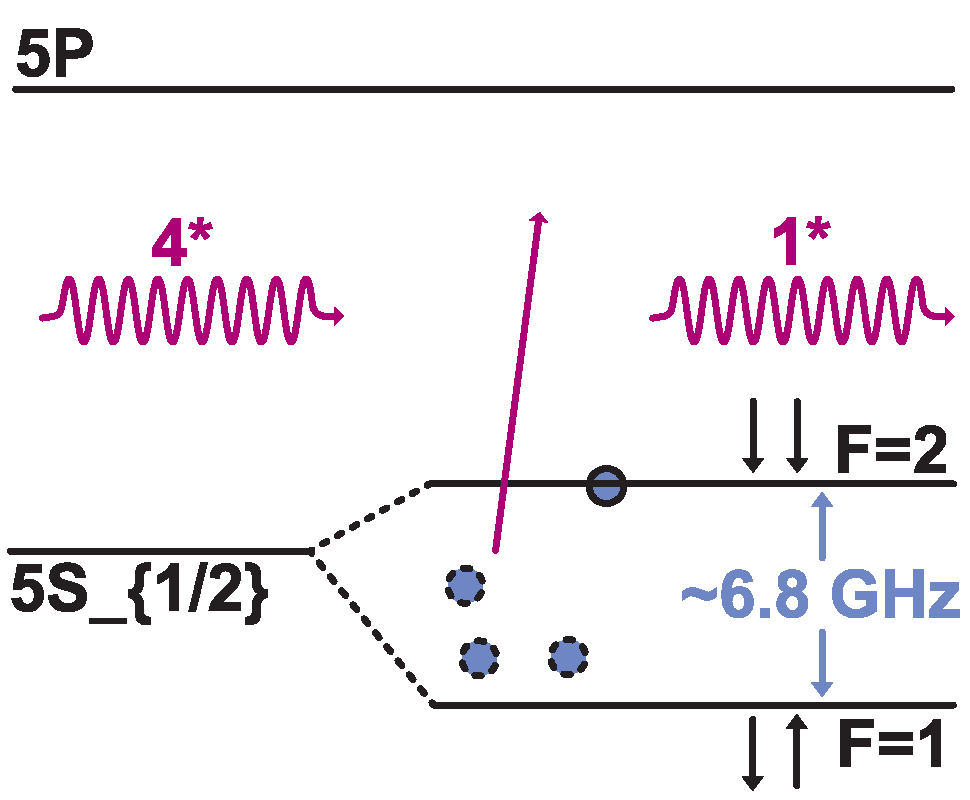
\includegraphics[width=\linewidth]{pdf/MODR/interrogation.pdf}
        \caption{Optical interrogation.}
        \label{fig:MODR-interrogation}
    \end{minipage}

    \caption{Electrons cycle in a MODR-based \acrshort{csac} due to the optical pumping, microwave excitation, and optical interrogation.}
    \label{fig:MODR-steps}
\end{figure}

With reference to Figure \ref{fig:MODR-steps}, we can now analyze deeper the different stages of the cycle and understand how it's possible to detect whether the microwave signal is in resonance with the atomic transition or not.

In particular, in Figure \ref{fig:MODR-pumping-decay} we can see four high energy photons coming from the pumping source that excite the electrons found at $5S_{1/2} F=1$, to $5^2P_{1/2}$ state.
From here, electrons will decay to both the $5^2S_{1/2} F=2$ and the $5^2S_{1/2} F=1$ states.
Over time however, the population will tend to accumulate on the $5^2P_{1/2} F=2$ state given that the excitation photons are not coupled with the \ref{itm:Rb-III} transition (due to the filter cell action).

During the second stage (Figure \ref{fig:MODR-microwave} for reference), the microwave excitation coming from the local oscillator is used to force the decay of the electrons from the $5^2S_{1/2} F=2$ state to the $5^2S_{1/2} F=1$ state.
Notice, however, that the decay is possible only if the microwave signal is at the right frequency of the transition, that is \ref{itm:Rb-I}.
In case the microwave signal is not exactly in resonance with the atomic transition, not all the electrons will be forced to decay and some of them will remain in the excited state.
Figure \ref{fig:MODR-microwave} shows an example where the microwave signal is not in perfect resonance with the atomic transition and 1 out of the 4 electrons remain in the $5^2S_{1/2} F=2$ state.

Finally, the cycle is closed with the interrogation phase (Figure \ref{fig:MODR-interrogation}).
Here, by sending the same amount of irradiation as in the pumping phase, we are able to detect if electrons are in the $5^2S_{1/2} F=1$ state or in the $5^2S_{1/2} F=2$ state.
In particular, in case not the entire population has decayed to the $5^2S_{1/2} F=1$ state during the microwave excitation, the interrogation phase will show a different intensity of the transmitted light.
In Figure \ref{fig:MODR-interrogation}, we can see that 1 out of the 4 photons will be transmitted given that only 3 atoms are in the $5^2S_{1/2} F=1$ state.

By measuring the intensity of the transmitted light, we can understand if the microwave signal was in resonance with the atomic transition or not.


\paragraph{Photodetector}

At the end of the vapor gas cell, a photodetector is used to measure the intensity of light transmitted through the reference cell.

In case of a MODR-based \acrshort{csac}, only if the microwave signal was in resonance with the atomic transition, most of the laser source from the bulb lamp will be absorbed by the atoms and the transmitted light will be minimal.
Conversely, in case of a non-resonant microwave signal, the intensity of the transmitted light will be stronger.

The signal captured by the photodetector is then sent to the control loop that will use it to fine-tune the local oscillator frequency.

\subsubsection{\acrfull{cpt}}
\label{sssec:CPT}

In case of a \acrfull{cpt} system, the physics package contains a vapor gas cell that receive a high energy signal from a laser source and force the valence electron of the \acrfull{cs} atoms to a coherent superposition of the two hyperfine ground states.
If this coherent superposition happens, the electron is said to be \textit{trapped in a dark state}, given that the incoming laser source will no more be coupled with the electron transitions and the atoms will not absorb the photons.

In a Physics Package based on \acrfull{cpt}, a vapor gas cell is irradiated by a highly modulated-circularly polarized laser source.
The laser source is modulated based on the local oscillator frequency.
Based on the effect of the laser source on the \acrfull{cs} atoms, we can understand whether the local oscillator is in resonance with the atomic transition frequency or not.

In order to better understand the operation of a CPT-based \acrshort{csac}, we leave here a schematic representation of its PP (Figure \ref{fig:CPT-physics-package-scheme}).

\begin{figure}[H]
    \centering
    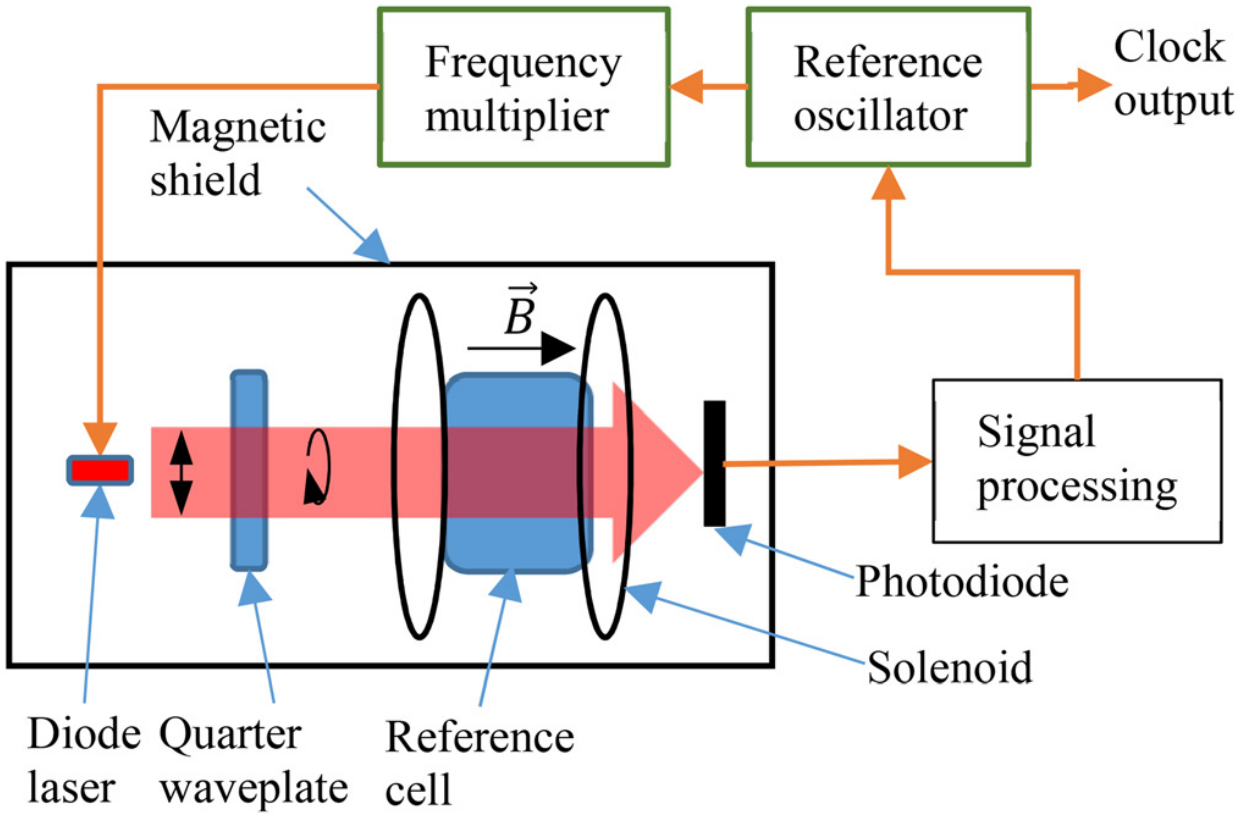
\includegraphics[width=0.6\textwidth, max width=\linewidth]{img/CPT-phisics-package-scheme.png}
    \caption{
        CPT-based \acrshort{csac} scheme.
        % Tha main components of the Physics Package are
    }
    \label{fig:CPT-physics-package-scheme}
\end{figure}

% MODR copy-paste
\paragraph{Target Electron Transitions of \acrfull{rb}}

In case of PP based on CPT, the vapor gas cell is typically filled with \acrfull{cs} ($^{133}Cs$) atoms.
$Cs$ is an alkaline metal with a relatively simple electronic structure, defined as $[Xe]6s^1$.
Its ionization energy is $3.894 eV$, and the valence electron can be exited using relatively low energy levels.
For these reasons, $Cs$ is widely used in atomic clocks, as it allows for precise manipulation of the valence electron while containing the energy required for the excitation.

In particular, by recalling the quantum energy levels of $^{133}Cs$ (defined by quantum effects and interactions between the electron and the nucleus), we can better define our working frame for the CPT architecture.
Three different transitions are of interest regarding the $^{133}Cs$ atom\footnote{In case of interest, a more comprehensive analysis of the $6S$ \& $6P$ energy levels of $^{133}Cs$ can be found in the Appendix \ref{appendix:Cesium-energy-levels}.}:

\begin{enumerate}[label = Cs.\Roman*, ref = Cs.\Roman*, leftmargin = *]
    \item \label{itm:Cs-I} $6^2S_{1/2} \quad F=3 \rightarrow 6^2S_{1/2} \quad F=4$: $\approx 9.2GHz$
    \item \label{itm:Cs-II} $6^2S_{1/2} \quad F=3 \rightarrow 6^2P_{1/2}$: $\approx 895^{-}nm$
    \item \label{itm:Cs-III} $6^2S_{1/2} \quad F=4 \rightarrow 6^2P_{1/2}$: $\approx 895^{+}nm$
\end{enumerate}

Notice that the transition $6^2S_{1/2} \rightarrow 6^2P_{1/2}$, of $\approx 895nm$, is usually refereed to as \textit{D1 line}.

\ref{itm:Cs-I}

\paragraph{Quantum Superposition}

Before moving on and understanding the different components of the CPT-based \acrshort{csac}, it's important to understand the concept of quantum superposition as it will be the key in the operation of the system.

In quantum mechanics, a quantum superposition is a fundamental principle that states that linear combinations of solutions to the Schr\"{o}dinger equation are also solutions of the Schr\"{o}dinger equation.
In other words, if $\ket{\psi_1}$ and $\ket{\psi_2}$ are solutions of the Schr\"{o}dinger equation, then $\alpha\ket{\psi_1} + \beta\ket{\psi_2}$ is also a valid solution of the state of the system.
A valid quantum superposition can be generally defined as:

\begin{equation}
    \ket{\psi} = c_\alpha\ket{\psi_\alpha} + c_\beta\ket{\psi_\beta}
\end{equation}

Where $\ket{\psi_\alpha}$ and $\ket{\psi_\beta}$ are two different states of the system and $c_\alpha$ and $c_\beta$ are complex numbers.
Practically speaking, this means that the electron can be found not only at the energy level associated with $\ket{\psi_\alpha}$ or $\ket{\psi_\beta}$, but also in a superposition of the two states (i.e. in any linear combination of the two states with a probability defined by the complex numbers).

To facilitate understanding of this counterintuitive concept, we report in the following two different interpretations of the quantum superposition:

\begin{itemize}
    \item Bloch Sphere representation: by imagining the electron as a 3D sphere with a finite radius, we can try to represent its energy level (i.e. its state) with a spatial vector with the origin in the center of the sphere and the tip on the surface. By mapping the ground state with an upward vector (Figure \ref{fig:Bloch-sphere-ground-state}) and the excited state with a downward vector (Figure \ref{fig:Bloch-sphere-excited-state}), we can intuitively understand that any other direction the vector might assume must be associated with a valid state of the electron. In other words, any other direction the state-vector other than the ground or the excited state is a valid quantum superposition that the electron can assume.
    \item Modal interpretation: given that to each energy level of the electron is associated a wave function, we can interpret the quantum superposition as a linear combination of the wave functions associated with the different energy levels. This interpretation derives from the approach used in classical vibrations problem, where the superposition of different modes (i.e. waves of different frequencies) can be used to describe the vibration of the system. In figure \ref{fig:modal-superposition}, we can see the superposition of two different modes that generate a new wave function.
\end{itemize}

\begin{figure}[H]
    \centering

    \begin{minipage}[t]{0.3\linewidth}
        \centering
        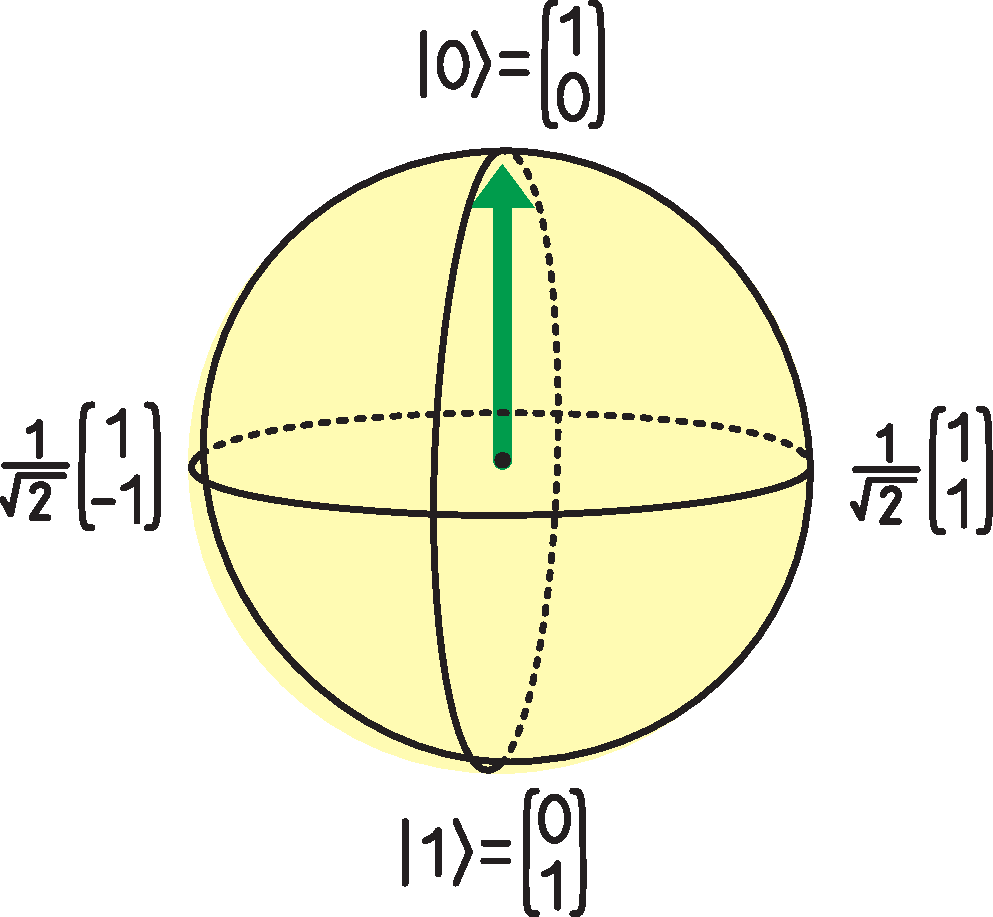
\includegraphics[width=\linewidth]{pdf/states/ground-state.pdf}
        \caption{Ground state.}
        \label{fig:Bloch-sphere-ground-state}
    \end{minipage}
    %
    \hfill
    %
    \begin{minipage}[t]{0.3\linewidth}
        \centering
        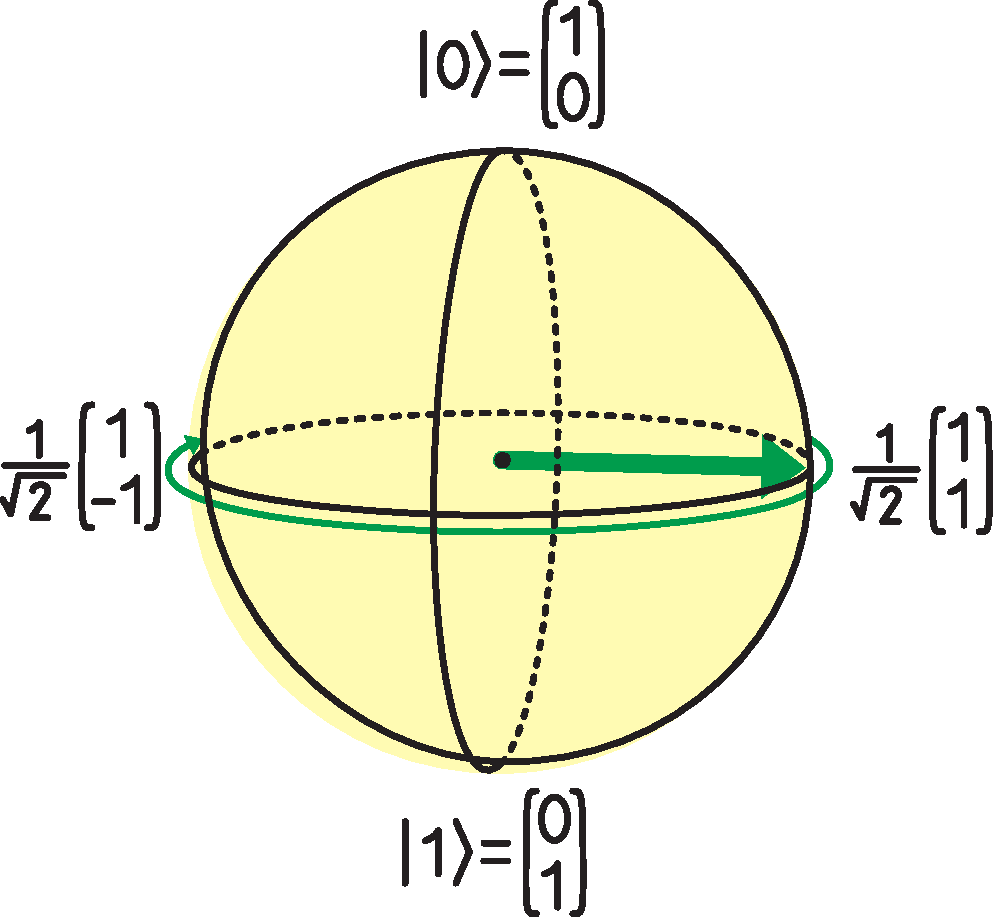
\includegraphics[width=\linewidth]{pdf/states/superposition-state.pdf}
        \caption{Superposition state.}
        \label{fig:Bloch-sphere-superposition}
    \end{minipage}
    %
    \hfill
    %
    \begin{minipage}[t]{0.3\linewidth}
        \centering
        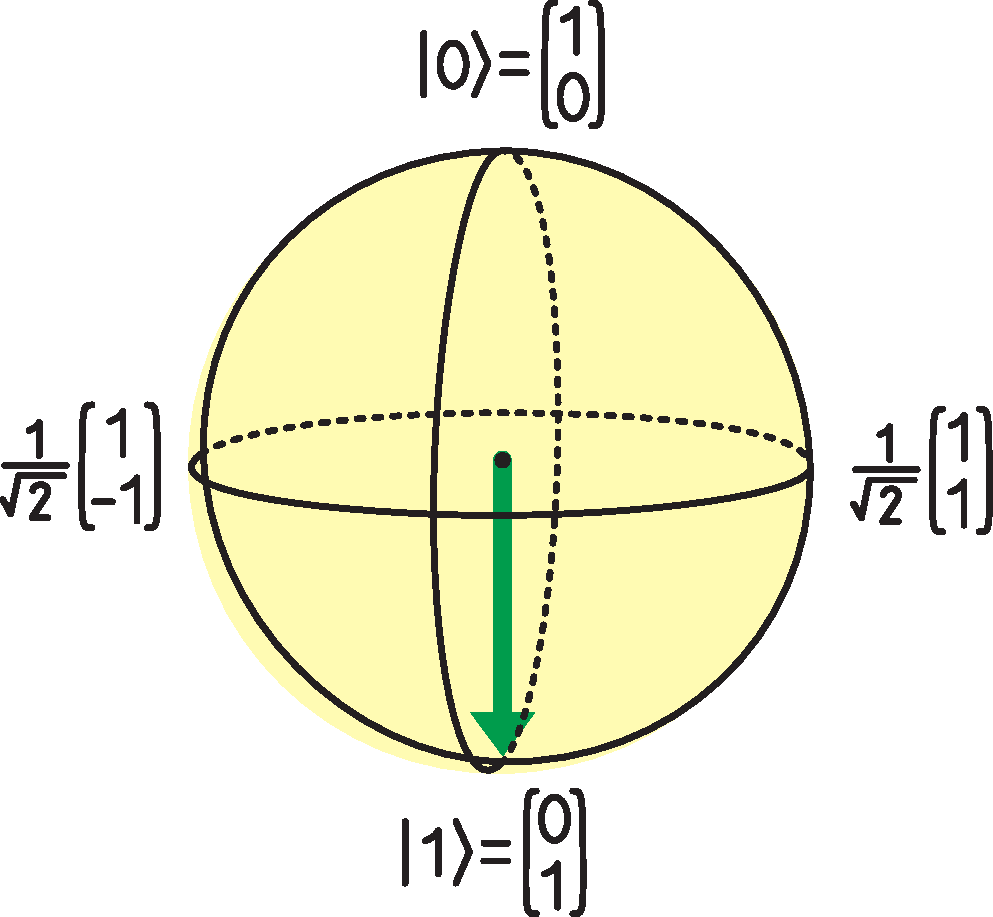
\includegraphics[width=\linewidth]{pdf/states/excited-state.pdf}
        \caption{Excited state.}
        \label{fig:Bloch-sphere-excited-state}
    \end{minipage}

    \caption{State superposition via Bloch sphere representation.}
    \label{fig:Bloch-sphere}
\end{figure}

\begin{figure}[H]
    \centering

    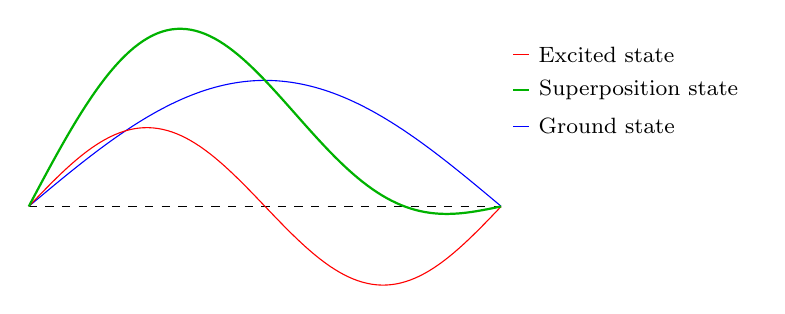
\begin{tikzpicture}

        \draw[dashed] (0, 0) -- (6, 0);

        \draw[blue, domain=0:6, samples=100] plot (\x, {1.6*sin(180/6*\x)});
        \draw[red, domain=0:6, samples=100] plot (\x, {1.0*sin(360/6*\x)});
        \draw[green!70!black, thick, domain=0:6, samples=100] plot (\x, {1.6*sin(180/6*\x) + 1.0*sin(360/6*\x)});

        % Add legend
        \node [matrix, font = \footnotesize, below right, row sep = 0cm] at (current bounding box.north east)
        {
            \draw[red] (0, 0) -- ++(0.2, 0) node[right, black] {Excited state}; \\
            \draw[green!70!black, thick] (0, 0) -- ++(0.2, 0) node[right, black] {Superposition state}; \\
            \draw[blue] (0, 0) -- ++(0.2, 0) node[right, black] {Ground state}; \\
        };

    \end{tikzpicture}

    \caption{State superposition via modal interpretation and wave functions.}
    \label{fig:modal-superposition}
\end{figure}


\paragraph{$\Lambda$-Lambda System \& Dark State}

Having understood the concept of quantum superposition, we can proceed and understand how it's useful related to the operation of a CPT-based \acrshort{csac}.
To do so, we need to introduce the concept of $\Lambda$-Lambda system and dark state.

A $\Lambda$-Lambda system is a quantum system composed of three energy levels (see Figure \ref{fig:lambda-system} for reference), where not all the dipole transitions are allowed.
In particular:

\begin{figure}[H]
    \centering

    \begin{minipage}[c]{0.49\linewidth}
        \centering
        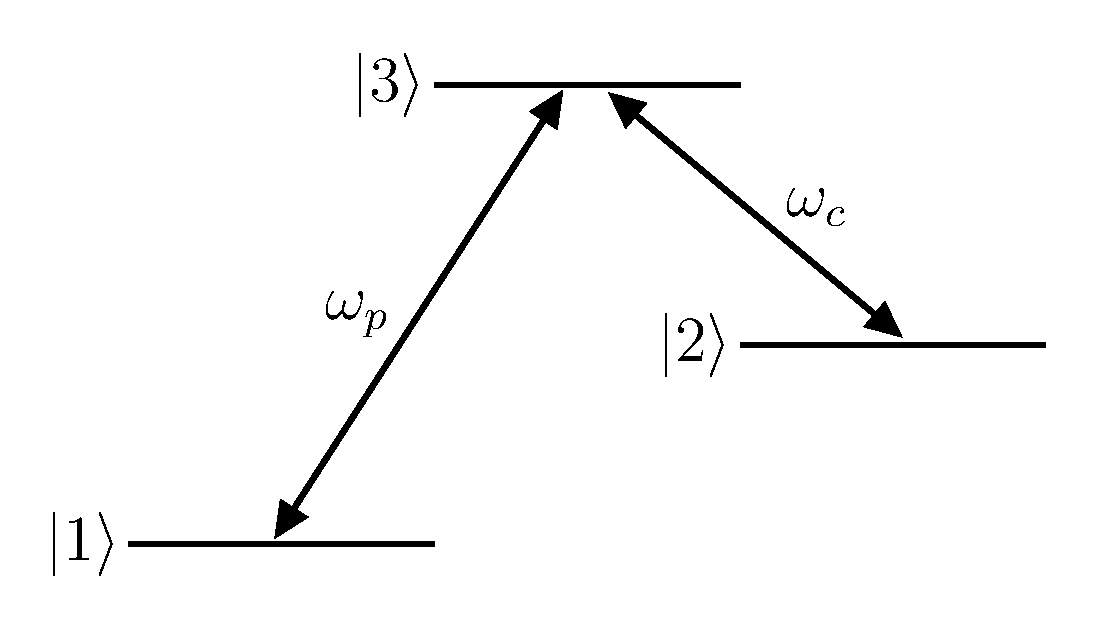
\includegraphics[width=\textwidth, max width=\linewidth]{pdf/lambda-system.pdf}
        \caption{$\Lambda$-system representation.}
        \label{fig:lambda-system}
    \end{minipage}
    %
    \hfill
    %
    \begin{minipage}[c]{0.49\linewidth}
        \begin{align}
            \text{Allowed transitions:}  & \begin{cases}
                                               \ket{1} \leftrightarrow \ket{3} \\
                                               \ket{2} \leftrightarrow \ket{3}
                                           \end{cases} \\
            \text{Forbidden transition:} & \begin{cases}
                                               \ket{1} \leftrightarrow \ket{2}
                                           \end{cases}
        \end{align}
    \end{minipage}

\end{figure}


In case the system is excited with a stable and well-controlled laser source (better explanation given in the following paragraph) that couples at the same time both the $\ket{1} \leftrightarrow \ket{3}$ and the $\ket{2} \leftrightarrow \ket{3}$ transitions, electrons will be pumped at first in their excited state (i.e. $\ket{3}$) and then forced to decay to $\ket{\psi}$, a superposition of $\ket{1}$ and $\ket{2}$.
This method is called \textit{coherent population trapping} and the system is said to be in a \textit{dark state} given that the incoming laser source will no more be coupled with the electron transitions and the atoms will not absorb the photons.

In our working frame, the $\Lambda$-system is composed of the two ground states $6^2S_{1/2} F=3$ \& $6^2S_{1/2} F=4$ and the excited state $6^2P_{1/2}$ of the $^{133}Cs$ atom.


\paragraph{Pumping Source}

From now on, given for granted the concept of quantum superposition and the $\Lambda$-system, we can step into understanding the components used to excite the $^{133}Cs$ atoms and obtain the desired dark state.

In a CPT-based \acrshort{csac}, the pumping source is typically a \textit{diode laser} (see Figure \ref{fig:CPT-physics-package-scheme} for reference), and most commonly a \textit{Vertical Cavity Surface Emitting Laser (VCSEL)}.
The use of a diode laser instead of a bulb lamp is due to the need of a stable and well-controlled source of irradiation that can be precisely modulated based on the local oscillator frequency.
In fact, VCSEL is a semiconductor laser diode that emits light from its top surface and it's characterized by a very narrow emission spectrum and a high modulation bandwidth.

In the framework of a CPT-based \acrshort{csac}, the diode laser is driven by the local oscillator frequency and it's modulated in both Amplitude (AM) and Frequency (FM).
In particular, in order to obtain the desired effect of coherent population trapping inside the reference cell, the laser source must met the following requirements:

\begin{itemize}
    \item AM modulation: the signal generated via the AM modulation must be at frequency \ref{itm:Cs-I} (i.e. the transition frequency of the $^{133}Cs$ ground states hyperfine splitting);
    \item FM modulation: the signal generated via the FM modulation must be at frequency of the \textit{D1 line} (i.e. the transition frequency of the $^{133}Cs$ ground state to the $^{133}Cs$ excited state).
    \item Circular polarization: the laser source must be positively circularly polarized.
\end{itemize}

The first two requirements can be easily met by controlling the injection current of the diode laser in time and are equivalent to state that the laser source must be the sum of a signal modulated at \ref{itm:Cs-II} with another modulated at \ref{itm:Cs-III} frequency.
In other words, the laser source must be able to generate the beating wave of the two frequencies as shown in Figure \ref{fig:beating-wave}.
The third requirement can be met by using a quarter-wave plate in front of the laser source that convert the linear polarization of the source in a circular one (again, see Figure \ref{fig:CPT-physics-package-scheme} for reference).

\begin{figure}[H]
    \centering

    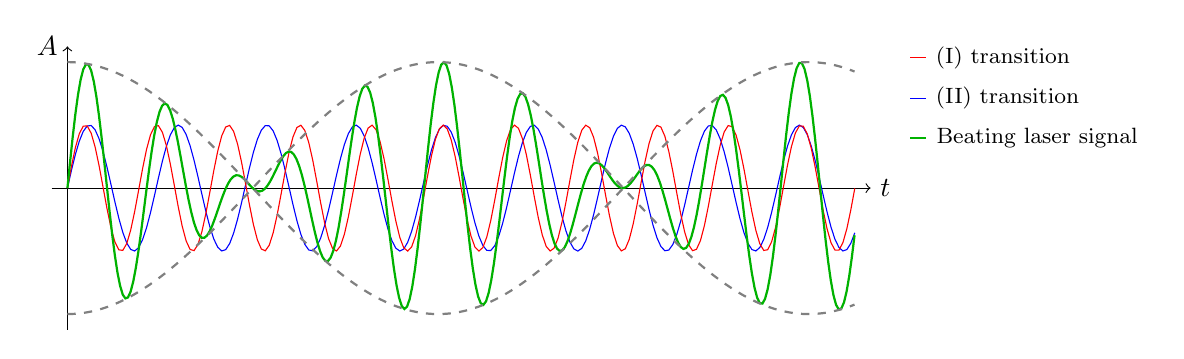
\begin{tikzpicture}
        \def\fa{1.775/2}
        \def\fb{2.20/2}
        \def\xmax{10}

        \draw[->] (-0.2, 0) -- (\xmax + 0.2, 0) node[right] {$t$};
        \draw[->] (0, -1.8) -- (0, 1.8) node[left] {$A$};

        \draw[blue, domain=0:\xmax, samples=200] plot (\x, {0.8*sin(360*\fa*\x)});
        \draw[red, domain=0:\xmax, samples=200] plot (\x, {0.8*sin(360*\fb*\x)});
        \draw[green!70!black, thick, domain=0:\xmax, samples=300] plot (\x, {0.8*sin(360*\fa*\x) + 0.8*sin(360*\fb*\x)});
        \draw[gray, thick, dashed, domain=0:\xmax, samples=300] plot(\x,{ 1.6*cos(180*(\fa-\fb)*\x)});
        \draw[gray, thick, dashed, domain=0:\xmax, samples=300] plot(\x,{ -1.6*cos(180*(\fa-\fb)*\x)});

        % Add legend
        \node [matrix, font = \footnotesize, below right, row sep = 0cm] at (current bounding box.north east)
        {
            \draw[red] (0, 0) -- ++(0.2, 0) node[right, black] {\textrm{(I)} transition}; \\
            \draw[blue] (0, 0) -- ++(0.2, 0) node[right, black] {\textrm{(II)} transition}; \\
            \draw[green!70!black, thick] (0, 0) -- ++(0.2, 0) node[right, black] {Beating laser signal}; \\
        };

    \end{tikzpicture}

    \caption{Beating wave of the laser source in a CPT-based \acrshort{csac} (AM modulation is highlighted with a dashed gray line, FM modulation is clearly visible on the green wave).}
    \label{fig:beating-wave}
\end{figure}

Notice, however, that the one represented in Figure \ref{fig:beating-wave} is the ideal case where the laser source is perfectly modulated at the two frequencies \ref{itm:Cs-II} and \ref{itm:Cs-III}.
In reality, the laser source is driven by the local oscillator frequency and some modulation errors will appear.
Those shift with respect to the ideal case will give us the information needed to understand if the local oscillator is in resonance with the atomic transition or not (i.e. if the local oscillator is at the right frequency or not).

\paragraph{Electrons Excitation and Interrogation}

Having understood what is the excitation source, we can now proceed understanding how this energy is used over the atoms present in the \textit{reference cell} (see Figure \ref{fig:CPT-physics-package-scheme}, also refereed to as \textit{vapor gas cell}) and in particular what's the cycle that electrons are forced to.

For the simplicity of the explanation, we will consider the different stages of the electrons as if they happen in a temporal sequence.
However, it's important to remind those stages are not sequential but they simultaneously happen.

We can define three different stages in the cycle of the electrons:

\begin{itemize}
    \item Optical pumping (population inversion): the laser source coming from the diode laser excites the atoms from both the $6S_{1/2} F=3$ and the $6S_{1/2} F=4$ ground hyperfine states to the $6^2P_{1/2}$ excited state.
    \item Decay to the dark state (superposition state): if the laser source during the pumping stage is modulated properly as described in the previous paragraph, then the excited electrons will now decay to a coherent superposition of the two ground states $6S_{1/2} F=3$ and $6S_{1/2} F=4$. The atoms are now in a dark state.
    \item Optical pumping (interrogation): the same laser used for population inversion is now used to interrogate the atoms and understand if the local oscillator frequency was in resonance with the atomic transition \ref{itm:Cs-I} or not.
\end{itemize}

To better understand the cycle of the electrons, we can refer to Figure \ref{fig:CPT-steps}.

\begin{figure}[H]
    \centering

    \begin{minipage}[t]{0.3\linewidth}
        \centering
        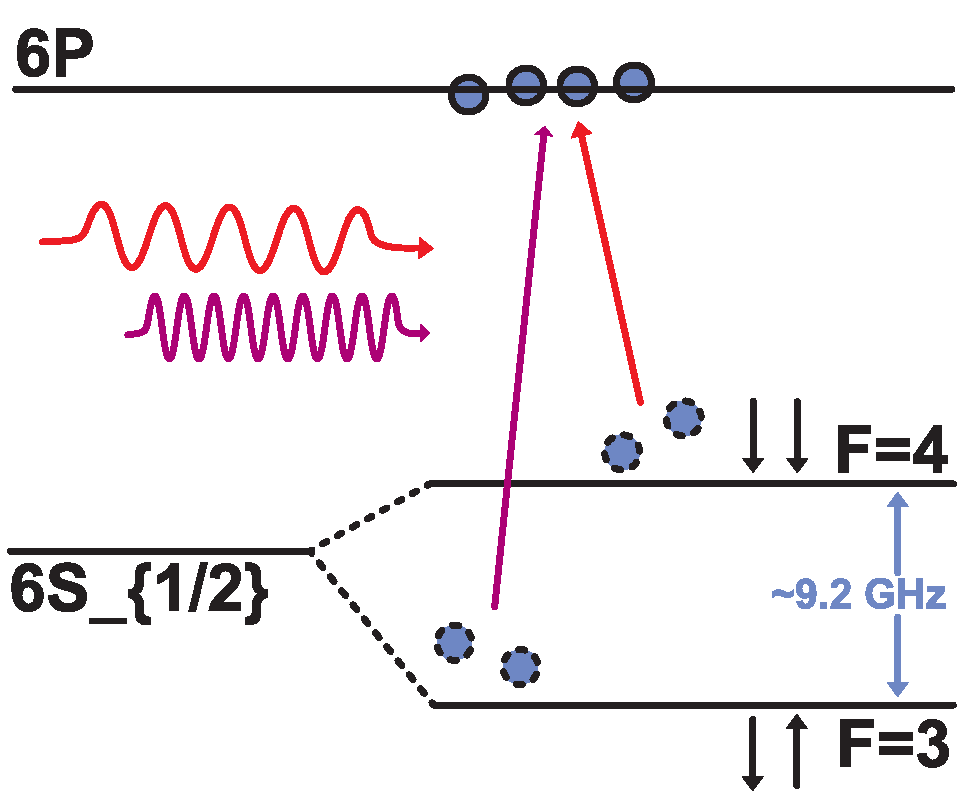
\includegraphics[width=\linewidth]{pdf/CPT/pumping.pdf}
        \caption{Population inversion.}
        \label{fig:CPT-pumping}
    \end{minipage}
    %
    \hfill
    %
    \begin{minipage}[t]{0.3\linewidth}
        \centering
        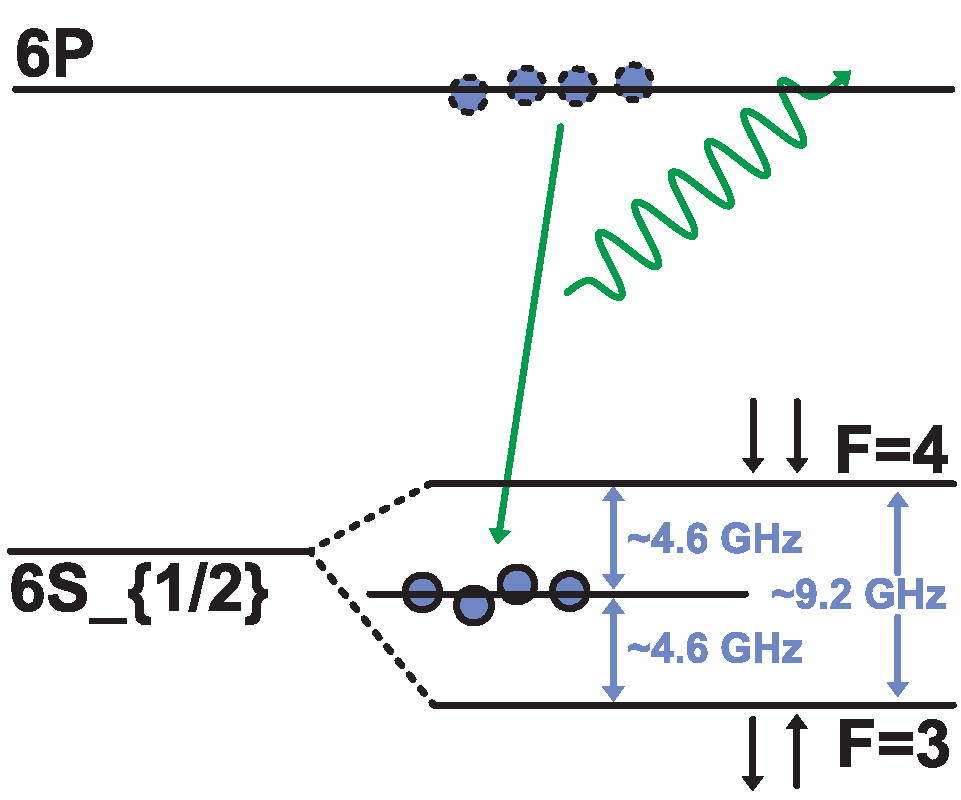
\includegraphics[width=\linewidth]{pdf/CPT/decay.pdf}
        \caption{Population decay.}
        \label{fig:CPT-decay}
    \end{minipage}
    %
    \hfill
    %
    \begin{minipage}[t]{0.3\linewidth}
        \centering
        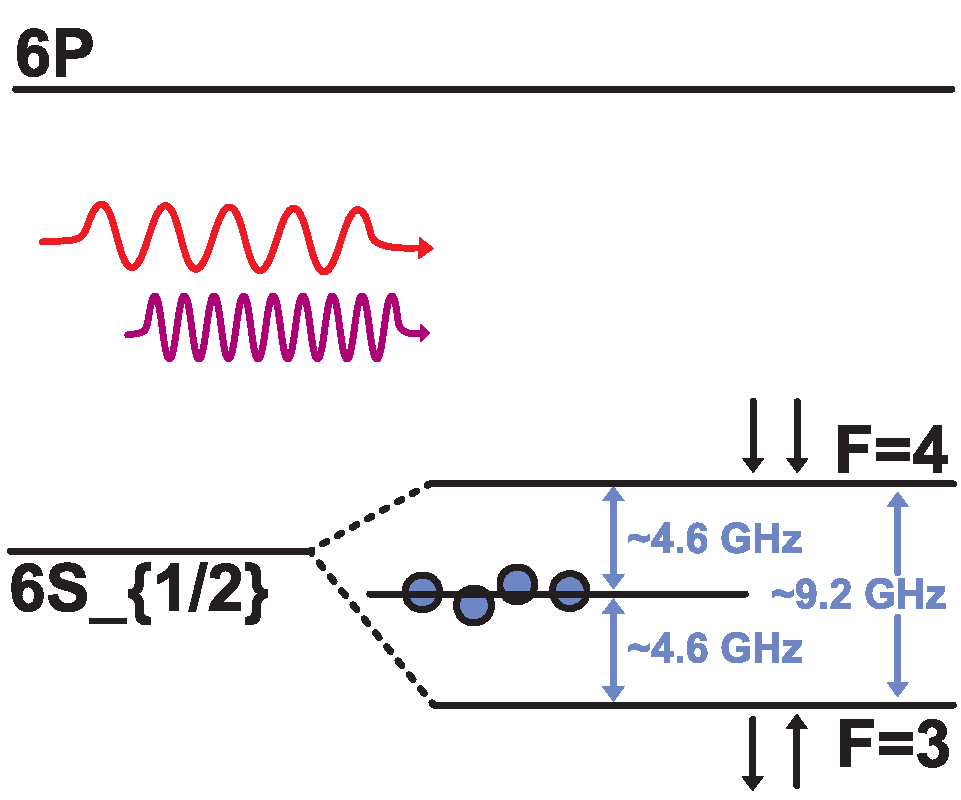
\includegraphics[width=\linewidth]{pdf/CPT/interrogation.pdf}
        \caption{Optical interrogation.}
        \label{fig:CPT-interrogation}
    \end{minipage}

    \caption{Electrons cycle in a CPT-based \acrshort{csac} due to the optical pumping, decay and optical interrogation.}
    \label{fig:CPT-steps}
\end{figure}

With reference to Figure \ref{fig:CPT-steps}, we can now analyze deeper the different stages of the cycle and understand how it's possible to detect whether the local oscillator is in resonance with the atomic transition or not.

For the sake of the explanation and simplification, we will consider the pumping laser source (the on coming from the diode laser) as two separate signals: one modulated at the frequency of the transition \ref{itm:Cs-II} and the other modulated at the frequency of the transition \ref{itm:Cs-III}.
In reality, the laser source is a beating wave of the two frequencies as shown in Figure \ref{fig:beating-wave}.
In Figure \ref{fig:CPT-pumping}, we can see four electrons that get excited from the $6S_{1/2} F=3$ and the $6S_{1/2} F=4$ ground hyperfine states to the $6^2P_{1/2}$ excited state.

Being $6^2P_{1/2}$ an unstable state, the electrons will start to decay to the non-excited states.
However, if the pumping laser source was modulated properly during the pumping stage, the electrons will now start to decay not only to both $6S_{1/2} F=3$ and $6S_{1/2} F=4$ states, but also to superposition state of the two.
In Figure \ref{fig:CPT-decay}, we can see that over time the population will tend to accumulate in a coherent superposition of the two ground states, given that from here the electrons won't be excited by the laser source and are said to be trapped.
Notice however, that the accumulation in the superposition state is possible only if the laser source was pumping at the right frequency, that is equivalent to say that the local oscillator was in resonance with the atomic transition \ref{itm:Cs-I}.

Finally, the cycle is closed with the interrogation phase (Figure \ref{fig:CPT-interrogation}).
Here, by sending the same amount of irradiation as in the pumping phase, we are able to detect if electrons are in one of the two ground states or in the superposition state.
In particular, in case not the entire population has decayed to the dark state during the decay, the interrogation phase will show a different intensity of the transmitted light.
In Figure \ref{fig:CPT-interrogation}, we can see that all the electrons are found in the superposition state and so the intensity of the transmitted light will be maximal since none of those electrons is coupled with the laser source.

By measuring the intensity of the transmitted light, we can understand if the local oscillator was in resonance with the atomic transition or not.


\paragraph{Photodetector}

At the end of the reference cell, a photodetector is used to measure the intensity of light transmitted through it.

In case of a CPT-based \acrshort{csac}, given that if the microwave signal was in resonance with the atomic transition, most of the laser source from the diode laser won't be anymore coupled to any electron, then the intensity of the transmitted light will be maximal.
Conversely, in case of a non-resonant microwave signal, the intensity of the transmitted light will be lower given that a fraction of the light will be absorbed by the electrons that are not in the superposition state.
In Figure \ref{fig:CPT-transmission}, we can see an example of a detuned signal captured by the photodetector.

\begin{figure}[H]
    \centering
    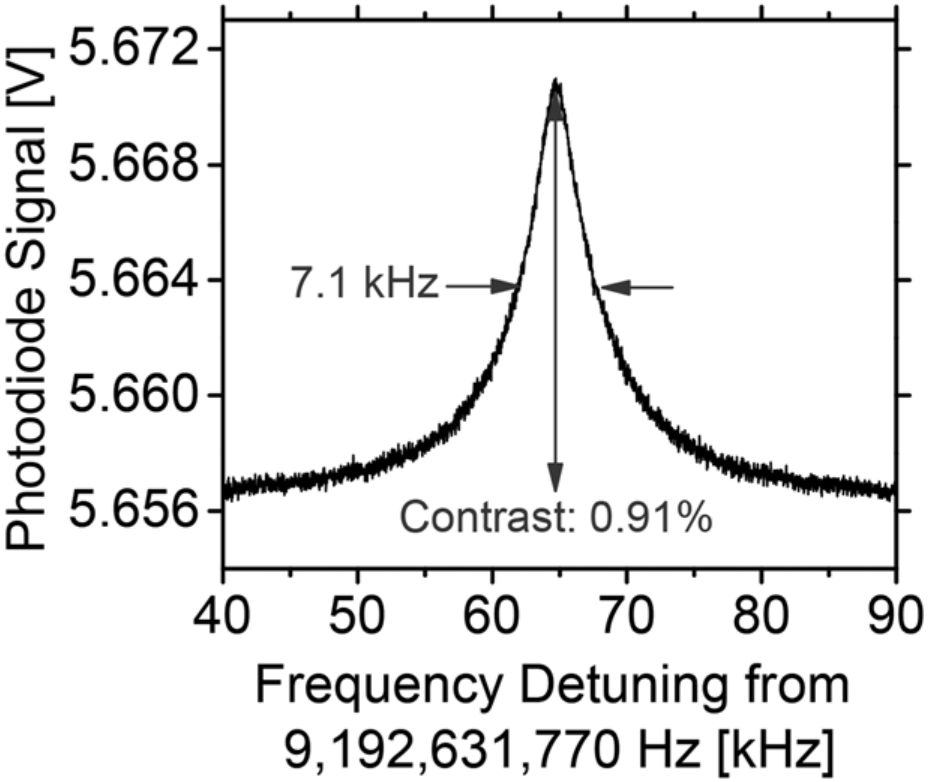
\includegraphics[width=0.5\textwidth, max width=0.8\linewidth]{img/CPT-transmission-signal.png}
    \caption{Detuned photodetection signal in a CPT-based \acrshort{csac}.}
    \label{fig:CPT-transmission}
\end{figure}

The signal captured by the photodetector is then sent to the control loop that will use it to fine-tune the local oscillator frequency (i.e. the clock frequency).


% TODO
\paragraph{Architecture Limitations}

Finally, we can move on and highlight the main limitations of a CPT-based \acrshort{csac} based on the metrics we have defined in Section \ref{sec:objective_metrics}.



\subsection{Control Loop (CL)}
\label{subsec:control_loop}

The \acrfull{cl} act as the brain of the clock, adjusting dynamically various parameters inside the \acrshort{csac} architecture to optimize stability and output frequency accuracy.
To do so, multiple servo loops based on PI\footnote{Proportional Integral} controllers are implemented to control specific areas and properties of different components. \acrshort{cl} takes as input the signal coming from the \acrfull{pp} and other sampled quantities coming from a network of sensors that are used to monitor the state of the clock (e.g., temperature sensors, magnetic field sensors, etc.)

\begin{figure}[H]
    \centering
    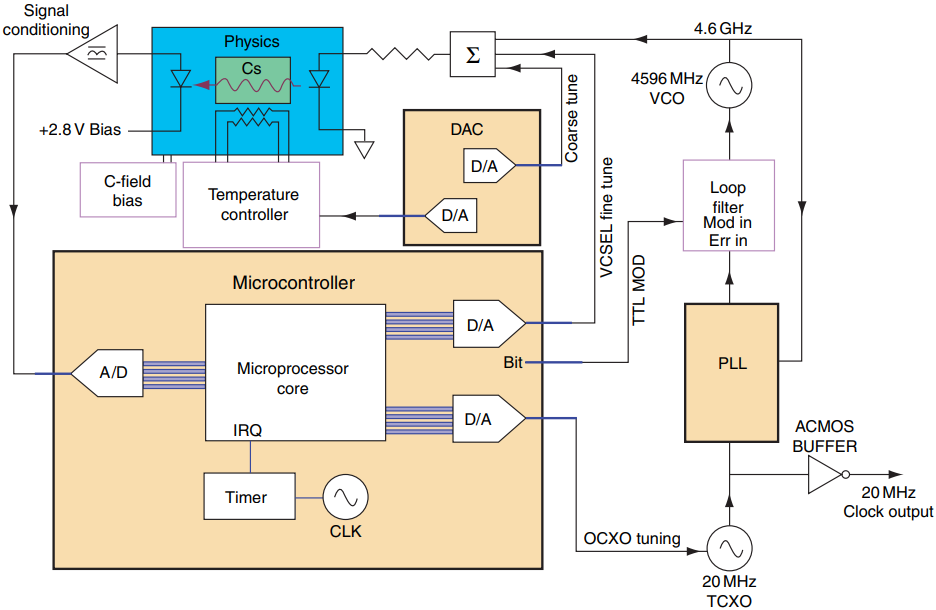
\includegraphics[width=.7\textwidth, max width=\linewidth]{img/control-loop.png}
    \caption{Control Loops block diagram for a CPT-based architecture (note the presence of the VCSEL). Source \cite{Knappe}.}
    \label{fig:control-loop}
\end{figure}

In Figure \ref{fig:control-loop} some key components are highlighted, such as microcontroller, converters (DAC and ADC), and PLL (Phase-Locked Loop) that are crucial for the correct functioning of the \acrshort{cl}.
In particular, the PLL is responsible for keeping in phase the \acrshort{lo} (indicated by the label "TCXO" in the bottom right) with the \acrshort{fs}, minimizing the phase noise and the frequency drift between the two components.

In a regular architecture, at least four servo loops are implemented to target different parameters.


\paragraph{Local Oscillator frequency servo loops}

The most important task of the \acrshort{cl} is the discipline of the \acrfull{lo} frequency to the desired value, locking it to the atomic resonance frequency or one of its multiple harmonics.

To achieve this, the \acrshort{cl} receives the output signal from the \acrshort{pp} and generate a feedback voltage signal that is sent to the \acrshort{lo} group.
Here, it's converted in a temperature variation of the crystal in order to modify its mechanical properties, thus adjusting the output frequency.

With reference to Figure \ref{fig:control-loop}, we can see this control line in the bottom right corner of the image, associated with the label "OCXO tuning", going from the microcontroller unit to the \acrshort{lo} group.

It has to be noted that the \acrshort{lo} has a much slower dynamics with respect to the electrical one provided by the microcontroller.
This causes an unavoidable delay over the feedback loop action and the actual effect on the \acrshort{lo} output frequency.


\paragraph{Laser frequency servo loops}

In case of the use of VCSEL as the excitation source, the \acrshort{cl} is also responsible for the control and tuning of its frequency that can be affected by external factors such as temperature variations or electrical/magnetic disturbances.

The diode laser is controlled by the summation of three different signal (see Figure \ref{fig:control-loop}), that are the coarse tune, the fine tune, and the \acrshort{fs} output.

In particular, the coarse tune signal is independent of any state of the clock and doesn't vary during the operation time.
The fine tune instead, is generated by the microcontroller and is used to compensate the environmental effects that cause a drift in the frequency of the excitation source.
Finally, the \acrshort{fs} output is added in order to permit the \acrshort{pp} to understand if the \acrshort{lo} is locked to the atomic resonance frequency.


\paragraph{Laser and cell temperature servo loops}

Maintaining constant temperatures for the laser and the reference cell within the \acrshort{pp} is another job of the \acrshort{cl}.

As we will see in the next section (Section \ref{sec:performances_and_limitations}), the temperature of these two components are crucial for the performances of the clock and should be maintained at a constant value during the operation time.

To do so, the feedback loop modify the temperature based on the signal coming from a network of thermocouple sensors that are placed near the targets.
Notice how, depending on the specific architecture of the clock, the \acrshort{cl} can act on the temperature of the two components independently or together.

In this way, the \acrshort{cl} ensures that both the excitation source and the atomic resonance frequencies are not affected by temperature variations, improving the photons coupling effectiveness.


\paragraph{Other servo loops}

In addition, other control loops can be implemented to target other parameters that might affect the performances of the clock.

Among these, one of particular importance is the servo used to shield or more in general control the magnetic field surrounding the \acrshort{pp}.
Again, with reference to Figure \ref{fig:control-loop}, we can recognize this control line in the bottom left corner of the "Physics" package block, associated with the label "C-field bias".

This control loop is used to maintain a zero or a constant value of the magnetic field inside the \acrshort{pp}, ensuring a precise and predictable behavior of the atomic resonance frequency that otherwise might suffer from frequency shifts (Zeeman and Stark effects, see Section \ref{sec:performances_and_limitations}).

\subsection{\acrfull{lo}}
\label{subsec:local_oscillator}